
\documentclass[10pt]{article}
\usepackage[a4paper,landscape,top=1.6cm,bottom=1.6cm,left=1.8cm,right=1.8cm]{geometry}
\usepackage[utf8]{inputenc}
\usepackage[T1]{fontenc}
\usepackage{lmodern}
\usepackage{microtype}
\usepackage{amsmath,amssymb}
\usepackage{xcolor}
\usepackage[most,breakable]{tcolorbox}
\usepackage{multicol}
\usepackage{booktabs,tabularx,longtable,array,colortbl}
\usepackage{fancyhdr}
\usepackage{enumitem}
\usepackage{lastpage}
\usepackage[hidelinks]{hyperref}
\usepackage{tikz}
\usetikzlibrary{arrows.meta,positioning,calc}
\definecolor{TealBg}{HTML}{E0F2F1}
\definecolor{NavyBg}{HTML}{E8EEFF}

\definecolor{Navy}{HTML}{0D2B6B}
\definecolor{Sky}{HTML}{1976D2}
\definecolor{Teal}{HTML}{00695C}
\definecolor{FGreen}{HTML}{2E7D32}
\definecolor{Amber}{HTML}{E65100}
\definecolor{DRed}{HTML}{B71C1C}
\definecolor{Purple}{HTML}{6A1B9A}
\definecolor{Indigo}{HTML}{303F9F}
\definecolor{LBg}{HTML}{F5F7FA}
\definecolor{BBg}{HTML}{E3F2FD}
\definecolor{GBg}{HTML}{E8F5E9}
\definecolor{RBg}{HTML}{FFEBEE}
\definecolor{ABg}{HTML}{FFF8E1}
\definecolor{IBg}{HTML}{E8EAF6}
\definecolor{TabOdd}{HTML}{EEF2F7}
\definecolor{TGcol}{HTML}{E65100}
\definecolor{QGcol}{HTML}{1565C0}
\definecolor{FGcol}{HTML}{2E7D32}

\tcbuselibrary{skins,breakable}
\tcbset{
  mybox/.style 2 args={
    enhanced, arc=3pt, boxrule=0.7pt,
    fonttitle=\bfseries\small\color{white},
    colbacktitle=#1, colframe=#1, colback=#2,
    lefttitle=5pt, toptitle=3pt, bottomtitle=3pt,
    top=5pt, bottom=5pt, left=6pt, right=6pt,
    before skip=5pt, after skip=5pt, breakable
  }
}
\newcommand{\navybox}[2]{\begin{tcolorbox}[mybox={Navy}{LBg},title={#1}]#2\end{tcolorbox}}
\newcommand{\skybox}[2]{\begin{tcolorbox}[mybox={Sky}{BBg},title={#1}]#2\end{tcolorbox}}
\newcommand{\tealbox}[2]{\begin{tcolorbox}[mybox={Teal}{LBg},title={#1}]#2\end{tcolorbox}}
\newcommand{\greenbox}[2]{\begin{tcolorbox}[mybox={FGreen}{GBg},title={#1}]#2\end{tcolorbox}}
\newcommand{\amberbox}[2]{\begin{tcolorbox}[mybox={Amber}{ABg},title={#1}]#2\end{tcolorbox}}
\newcommand{\redbox}[2]{\begin{tcolorbox}[mybox={DRed}{RBg},title={#1}]#2\end{tcolorbox}}
\newcommand{\purplebox}[2]{\begin{tcolorbox}[mybox={Purple}{LBg},title={#1}]#2\end{tcolorbox}}
\newcommand{\indigobox}[2]{\begin{tcolorbox}[mybox={Indigo}{IBg},title={#1}]#2\end{tcolorbox}}

\newcommand{\pagehead}[2]{%
  \begin{tcolorbox}[enhanced,arc=0pt,outer arc=0pt,boxrule=0pt,
    colback=Navy,colframe=Navy,
    top=5pt,bottom=5pt,left=8pt,right=8pt,
    before skip=0pt,after skip=10pt]
  {\color{white}\large\bfseries #1}%
  \ifx\relax#2\relax\else\\[1pt]{\color{blue!30!white}\small #2}\fi
  \hfill{\color{blue!20!white}\footnotesize Synthetic Financial Time Series $\cdot$ UPC}
  \end{tcolorbox}}

%% audit-row box (used in Extended Data)
\newcommand{\auditrow}[5]{%
  \begin{tcolorbox}[mybox={#2}{#3},
    title={\textbf{[#1]}\quad #4},
    before skip=4pt, after skip=4pt, breakable]
  \small #5
  \end{tcolorbox}}

\pagestyle{fancy}\fancyhf{}\renewcommand{\headrulewidth}{0pt}
\fancyfoot[C]{\small\color{gray!70}
  Page~\thepage\ of~\pageref{LastPage}\quad$\cdot$\quad
  Synthetic Financial Time Series --- GAN Benchmark\quad$\cdot$\quad UPC / BSE}

\newcommand{\tcite}[1]{%
  \hyperlink{R:#1}{\textsuperscript{\scriptsize\textbf{[#1]}}}}

\setlength{\parindent}{0pt}\setlength{\parskip}{4pt}\setlength{\columnsep}{14pt}
\setlist[itemize]{noitemsep,topsep=2pt,leftmargin=14pt,label=\textbullet}
\setlist[enumerate]{noitemsep,topsep=2pt,leftmargin=16pt}
\newcommand{\E}{\mathbb{E}}
\newcommand{\norm}[1]{\left\|#1\right\|}

%% ═══════════════════════════════════════════════════════════════════════════════
\begin{document}

%% ─── Page 1: Title ───────────────────────────────────────────────────────────
\thispagestyle{empty}
\pagecolor{Navy}\color{white}
\vspace*{2.0cm}
\begin{center}
{\fontsize{26}{32}\selectfont\bfseries Synthetic Financial Time Series Generation\par}
\vspace{0.4cm}
{\Large GAN Benchmark:\quad TimeGAN\ \ $\cdot$\ \ QuantGAN\ \ $\cdot$\ \ FinGAN\par}
\vspace{0.2cm}
{\large BRICS Emerging Market Indices\par}
\vspace{0.7cm}
\textcolor{blue!40!white}{\rule{0.65\textwidth}{0.5pt}}
\vspace{0.7cm}

\begin{tabular}{r@{\hspace{10pt}}l}
  \textbf{Format}        & Dual-audience: Foundations (Part~I) $\cdot$ NMI Technical (Part~II) \\[4pt]
  \textbf{Collaboration} & Universitat Polit\`{e}cnica de Catalunya (UPC) \\[4pt]
  \textbf{Document type} & Research draft --- NMI-format submission in preparation \\[4pt]
  \textbf{Models}        & TimeGAN (GRU) $\cdot$ QuantGAN (TCN-WGAN-GP) $\cdot$ FinGAN (CNN-WGAN-GP) \\[4pt]
  \textbf{Markets}       & BOVESPA $\cdot$ FTSE JSE $\cdot$ MSCI $\cdot$ NIFTY50 $\cdot$ SHANGHAI \\[4pt]
  \textbf{Generated}     & 2026-08-30 \\
\end{tabular}
\end{center}
\clearpage\pagecolor{white}\color{black}

%% ═══════════════════════════════════════════════════════════════════════════════
%% PART I — FOUNDATIONS
%% Target reader: intelligent 13-year-old. Arithmetic only. No Greek letters
%% without an everyday anchor. No forward references.
%% ═══════════════════════════════════════════════════════════════════════════════

%% ─── Page 2: Summary + Sections 1–2 ─────────────────────────────────────────
\pagehead{Summary --- For All Readers}
         {Non-specialist language $\cdot$ $\leq$200 words $\cdot$ required by Nature Machine Intelligence}

\begin{tcolorbox}[enhanced,arc=4pt,boxrule=1pt,colframe=Teal,colback=TealBg,
  top=6pt,bottom=6pt,left=8pt,right=8pt,before skip=4pt,after skip=8pt]
\small
Markets generate data about themselves every day --- prices rising and falling --- but this data is scarce, expensive, and legally sensitive.
We trained three artificial-intelligence systems on five emerging financial markets (Brazil, South Africa, the MSCI index, India, and China) to generate convincing fake market data.

The core difficulty is that fake market data looks easy to evaluate but is not.
We discovered that a simple shuffled copy of real data --- identical individual values, wrong ordering --- passed nine of our sixteen quality tests with a perfect score.
This finding reshaped our evaluation from a single score into two families: nine tests for whether the individual numbers look right, and seven tests for whether the ordering looks right.

Across all three AI systems and five markets, the ordering tests proved the hardest to satisfy.
No generator fully reproduced the tendency of turbulent days to cluster together --- a property that matters critically for risk management.

We release all code and evaluation pipelines so others can apply the same tests to future generators on any market.
\end{tcolorbox}

\vspace{4pt}
\begin{tcolorbox}[enhanced,arc=0pt,outer arc=0pt,boxrule=0pt,
  colback=Navy!10,colframe=Navy!10,top=3pt,bottom=3pt,left=8pt,right=8pt]
{\large\bfseries\color{Navy} PART I --- FOUNDATIONS}
\hfill{\small\color{Navy!70} Sections 1--9\quad$\cdot$\quad No calculus\quad$\cdot$\quad Arithmetic only}
\end{tcolorbox}

\begin{multicols}{2}

\navybox{1\quad What We Are Trying to Build}{%
Imagine you work at a bank. You need to test your risk systems. Those systems are built to survive crashes --- the kind of day when markets fall 5\% or more. But crashes are rare by definition. Real history gives you only a handful of them.

What you actually need is a machine that can generate \emph{thousands} of plausible market histories, including many crashes, so you can stress-test your systems properly.

That machine is what this project builds. Specifically, we train three different artificial-intelligence programs to learn from five years of real daily market data from five emerging economies. Each program learns what a realistic market day looks like --- how volatile, how skewed, how connected to the day before. Then it generates as many fake days as we need.

The word for such a program is a \textbf{generative model}. The specific type we test is called a \textbf{Generative Adversarial Network} (GAN), first proposed by Goodfellow et al.\ (2014)\tcite{1}.

\smallskip
\textit{This analogy stops working when:} a bank stress-test is a controlled simulation; real markets respond to the tests themselves, which no generative model captures.}

\columnbreak

\navybox{2\quad Prices, and Why We Study Changes}{%
A stock index on Monday might be 4{,}000. On Tuesday, 4{,}080. On Wednesday, 4{,}050. These raw numbers grow over decades and shrink during crashes. They are hard to compare across markets or time periods.

Instead we compute the \textbf{log return} for each day:
\begin{equation*}
  r_t = \ln\!\left(\frac{P_t}{P_{t-1}}\right)
\end{equation*}

\textbf{Worked arithmetic.} Monday to Tuesday: $\ln(4080/4000) = \ln(1.02) \approx 0.0198$. That is a return of roughly $2\%$. Tuesday to Wednesday: $\ln(4050/4080) \approx -0.0074$, a drop of $0.74\%$.

Two useful properties make log returns the standard choice.
First, returns from different days can simply be added: a $2\%$ gain followed by a $-0.74\%$ drop gives a total of $1.26\%$, which is close to the actual $\ln(4050/4000) \approx 1.24\%$ (the small gap shrinks for smaller moves).
Second, log returns fluctuate around zero with no long-run trend, which is what the AI systems need to learn from.

\smallskip
Going forward, every number we call a ``market value'' is a daily log return. The typical size of a daily return in our five markets is about $1\%$.}

\end{multicols}

\clearpage

%% ─── Page 3: Sections 3–4 (the two worked examples) ────────────────────────
\pagehead{Part I --- Foundations (continued)}
         {The two properties of real markets that most generators fail to reproduce}

\begin{multicols}{2}

\redbox{3\quad The Bell Curve Fails}{%
Suppose you measure the height of every student in a large school. Almost everyone lands near the average. A few are much taller, a few much shorter, and nobody is three metres tall. Heights follow the shape people call a \textbf{bell curve}: a big lump in the middle, thin tails at the edges.

For two centuries, mathematicians assumed the ups and downs of stock prices behaved the same way. It is a reasonable guess. It is also wrong, and the way it is wrong matters enormously.

\medskip
\textbf{Here is the arithmetic.} In our five markets, a typical day moves the index by about $1\%$. Call that one ``step''. The bell curve makes a very specific promise about rare events: a day that moves five steps --- a $5\%$ jump or crash --- should happen roughly \textbf{once every 6,922 years}.

We looked at five markets over five years. That is about 6,201 market-days in total. The bell curve predicts we should see essentially zero such days.

\medskip
We found \textbf{11}.

\medskip
This is not a small error. It is not a matter of the model being slightly off. Reality delivered extreme days thousands of times more often than the bell curve allows. The Shanghai index alone had five such days in five years.

That gap is why this project exists. If you are a bank estimating your worst plausible loss, and your model says a $5\%$ crash arrives once per 6,922 years while reality delivers one every few years, you are not slightly wrong. You are unprepared.

Professionals call this property \textbf{heavy tails} --- the ``tails'' being the far edges of the curve, and ``heavy'' meaning there is more weight out there than the bell curve predicts. The number that measures it is called \textbf{kurtosis}. A bell curve scores~0. Our five markets score between 1.1 and 9.1, all above zero, all confirming the same thing.

\smallskip
\textit{Where this analogy stops working:} human heights genuinely do follow a bell curve, and no student will ever be three metres tall. Market returns have no such ceiling. That is precisely the difference.}

\columnbreak

\amberbox{4\quad Storms Cluster}{%
Think about weather. Rainy days are not scattered randomly through the year. Rain comes in stretches. If it poured yesterday, it is more likely to pour today --- not certain, just more likely. Storms arrive in clusters.

Markets do the same thing, and we can measure it exactly. Take the MSCI index. On any given day, there is a $5.0\%$ chance of a ``big move'' --- one at least twice the size of a typical day.

Now ask a different question: given that yesterday \emph{was} a big move, what is the chance today is too?

\medskip
The answer is $\mathbf{11.1\%}$.

\medskip
That is \textbf{2.21 times higher}. Turbulence begets turbulence.

This creates a trap for anyone building a fake market. You could construct a series that gets the bell-curve shape exactly right --- the correct number of calm days, the correct number of wild days, the correct heavy tails --- and still be completely wrong, because you scattered the wild days randomly instead of letting them cluster.

We tested exactly this. We took real market data and shuffled it, like shuffling a deck of cards. Shuffling changes nothing about \emph{how many} big days there are --- every day is still there, just in a different order. It only destroys \emph{when} they happen.

Then we ran our quality tests on the shuffled version. Four of our six main distributional tests gave it a \textbf{perfect score}.

That result reshaped this project. It means the standard way of checking synthetic market data cannot tell the difference between a good model and a shuffled deck of cards. Most of our work has gone into fixing that.

\smallskip
\textit{Where this analogy stops working:} weather clustering is driven by physical systems moving across a map. Market clustering comes from human behaviour --- fear spreading, positions unwinding, margin calls. Same pattern, different engine.}

\end{multicols}

\clearpage

%% ─── Page 4: Sections 5–7 ───────────────────────────────────────────────────
\pagehead{Part I --- Foundations (continued)}
         {Why synthetic data matters $\cdot$ why judging it is hard $\cdot$ the shuffled-deck discovery}

\begin{multicols}{2}

\skybox{5\quad Why Anyone Wants Synthetic Markets}{%
If real data exists, why generate fake data? There are three reasons, each pointing at a different kind of problem.

\medskip
\textbf{Reason 1: not enough real crashes.} Deep learning systems need thousands of examples to learn reliably. Real markets produce roughly 250 trading days per year. A five-year dataset gives 1{,}250 days. A single crash, by definition, happens rarely --- so the system trains on almost none of them. A generative model can supply as many fake crash sequences as needed.

\medskip
\textbf{Reason 2: stress testing.} Banks and regulators must demonstrate that their risk systems survive scenarios that have not happened yet. ``What would a 2008-style crisis look like in the Brazilian market?'' Real history cannot answer that. A well-trained generator can produce thousands of plausible answers.

\medskip
\textbf{Reason 3: sharing without revealing secrets.} Real trading data is often proprietary. A hedge fund cannot share its positions. A central bank cannot share its internal stress scenarios. Synthetic data with the same statistical properties can be released freely, enabling research that would otherwise be impossible.

\smallskip
The challenge in all three cases is the same: the fake data must be \emph{good enough to use}. A model that produces the right average daily move but scatters the wild days randomly is useless for stress testing --- it has already failed the clustering test from Section~4.}

\skybox{6\quad Why Judging It Is Hard}{%
The obvious test is: ``does this look real?'' But ``looking real'' turns out to be surprisingly hard to measure.

The most common test in statistics --- the Kolmogorov-Smirnov test --- was designed for situations where each measurement is independent of the others. Coin flips are independent. Market returns are not: today's volatility is correlated with yesterday's (Section~4). When you run the KS test on correlated data, it systematically over-rejects even good generators.

Another common test --- mean squared error --- compares the $t$-th real return to the $t$-th synthetic return. But a real series and a synthetic series are independently generated. There is no reason why the 47th fake day should correspond to the 47th real day. Comparing them directly measures nothing meaningful.

The metric that works better is the \textbf{Wasserstein distance}: imagine the real returns as a pile of sand and the synthetic returns as another pile. The Wasserstein distance is the minimum total work needed to reshape one pile into the other --- weight times distance, summed over every grain. Unlike the KS test, it remains meaningful even when the data is not independent.

But even Wasserstein has a blind spot, which the next section reveals.}

\columnbreak

\redbox{7\quad The Shuffled Deck --- What We Discovered}{%
We built a simple adversarial test. Take the real BRICS test data. Shuffle it randomly --- like shuffling a deck of cards, as described in Section~4. The shuffled version has \emph{identical} individual values: same histogram, same average, same heavy tails, same kurtosis. It destroys only the ordering.

Then we ran every quality test on this shuffled control.

\medskip
\begin{tabular}{@{}lc@{}}
\toprule
Test & Shuffled control score \\
\midrule
KS statistic   & \textbf{0.000000} (perfect) \\
Wasserstein    & \textbf{0.000e+00} (perfect) \\
kurtosis diff  & \textbf{1.78e-15} (perfect) \\
energy distance & \textbf{2.97e-05} (perfect) \\
\midrule
ACF clustering & 0.0758 (correctly penalised) \\
Hurst diff     & 0.052 (correctly penalised) \\
\bottomrule
\end{tabular}

\medskip
Nine of the 19 metrics we had been ranking returned a perfect or near-perfect score for the shuffled control. When we computed the composite ranking --- average rank across all metrics --- the shuffled control \textbf{ranked first}, with avg\_rank 1.24 versus 2.47 for a real generator.

This result was not a bug. It was a diagnosis. It means that nine of our nineteen metrics are \emph{permutation-invariant} --- they measure the individual values only, not their order. A shuffled deck of cards scores perfectly on those nine tests because shuffling does not change which cards are in the deck.

Any composite score that mixes permutation-invariant and ordering-sensitive metrics without equal weighting will be dominated by the invariant ones. The control will always win on the invariant metrics, because it \emph{is} the real data in a different order.

\smallskip
This finding is the central methodological contribution of this paper.}

\end{multicols}

\clearpage

%% ─── Page 5: Sections 8–9 ───────────────────────────────────────────────────
\pagehead{Part I --- Foundations (continued)}
         {What we did about the shuffled-deck problem $\cdot$ what we still cannot do}

\begin{multicols}{2}

\tealbox{8\quad What We Did About It}{%
The shuffled-deck finding required three changes to the evaluation.

\medskip
\textbf{Change 1: split the metrics into two families.}

\textit{Fidelity metrics} (nine): these are the permutation-invariant tests that measure whether the individual values look right --- the right distribution, the right tails, the right kurtosis. Necessary but not sufficient. A shuffled deck passes all nine.

\textit{Temporal metrics} (seven): these are ordering-sensitive tests that measure whether the sequence behaves like a real market --- volatility clustering, long memory, conditional non-Gaussianity, and a classifier that tries to tell real from fake using the ordering of values. A shuffled deck fails all seven.

\medskip
\textbf{Change 2: give each family equal weight.}

The composite score is:
\begin{equation*}
  \text{composite\_rank} = \frac{\text{fidelity\_rank} + \text{temporal\_rank}}{2}
\end{equation*}

Nine fidelity metrics cannot outvote seven temporal ones. The families are what is weighted, not the individual metrics.

\medskip
\textbf{Change 3: exclude the control from the competition.}

No weighting scheme can prevent the shuffled control from winning on fidelity metrics. It is a permutation of the real data; it will always score perfectly on tests that ignore ordering.

The solution: compute ranks only among the three GAN generators. The shuffled control is appended to the results table with rank = NaN so readers can see what a marginal-only generator achieves --- and any generator that scores \emph{worse} than the control on temporal metrics has not learned anything about market dynamics.

\medskip
After these three changes, the final composite rankings are:

\begin{tabular}{@{}lcc@{}}
\toprule
Generator & fidelity\_rank & temporal\_rank \\
\midrule
real\_like (best)  & 1.44 & 1.29 \\
gaussian (wide)    & 1.56 & 1.71 \\
too\_wide          & 2.00 & 2.00 \\
\midrule
Control (reference) & --- & --- \\
\bottomrule
\end{tabular}

\smallskip
The best composite score is 1.421.}

\columnbreak

\purplebox{9\quad What We Still Cannot Do}{%
This project establishes a benchmark and evaluation framework. It does not solve the underlying problem completely. Four limitations matter for the paper.

\medskip
\textbf{Limitation 1: five years of data is short.}

The Hill estimator for tail heaviness has a standard deviation of 0.52 at $n=995$ (our per-market sample size), falling to 0.035 at $n=4{,}000$ --- a 15-fold improvement. With only five years of history, our tail estimates are noisy enough that two generators could swap positions just from sampling variation. Extending to 15--20 years of data would sharpen every temporal metric and is the highest-leverage remaining change.

\medskip
\textbf{Limitation 2: no diffusion model baseline.}

Takahashi and Mizuno (2025)\tcite{29} showed that diffusion-based generators outperform GANs on several stylized-fact metrics. Our benchmark covers three GAN architectures; it does not include a diffusion baseline. Reviewers will ask. The answer is: not yet.

\medskip
\textbf{Limitation 3: no systematic hyperparameter search.}

All three GAN architectures use reference-implementation defaults from their original papers. No search over learning rates, hidden dimensions, or noise dimensions has been run. TimeGAN in particular is trained with only five epochs --- far below the 5{,}000--10{,}000 iterations per phase recommended by Yoon et al.\ (2019)\tcite{4}. TimeGAN's poor ranking reflects this budget, not its architecture.

\medskip
\textbf{Limitation 4: ARCH tests are unreliable across regimes.}

The ARCH-LM test, the standard tool for detecting volatility clustering, saturates on real fat-tailed data (both real and shuffled series give $p$-value $= 0.0$, so the difference is $0.000000$). On simulated GARCH data it works well (99\% accuracy). But on real BRICS data it cannot distinguish a good generator from a shuffled deck. This limitation is itself a result, reported in Part~II.}

\end{multicols}

\clearpage

%% ═══════════════════════════════════════════════════════════════════════════════
%% PART II — TECHNICAL SPECIFICATION (NMI FORMAT)
%% ═══════════════════════════════════════════════════════════════════════════════

%% ─── Page 6: Abstract + Untitled Opening ─────────────────────────────────────

\begin{tcolorbox}[enhanced,arc=0pt,outer arc=0pt,boxrule=0pt,
  colback=Navy!10,colframe=Navy!10,top=3pt,bottom=3pt,left=8pt,right=8pt,
  before skip=0pt,after skip=6pt]
{\large\bfseries\color{Navy} PART II --- TECHNICAL SPECIFICATION}
\hfill{\small\color{Navy!70} NMI format $\cdot$ Abstract $\cdot$ Results $\cdot$ Discussion $\cdot$ References $\cdot$ Methods}
\end{tcolorbox}

\begin{tcolorbox}[enhanced,arc=4pt,boxrule=1pt,colframe=Navy,colback=LBg,
  top=6pt,bottom=6pt,left=8pt,right=8pt,before skip=2pt,after skip=8pt,
  title={\bfseries Abstract --- $\leq$150 words, unreferenced}]
\small
We benchmark three generative adversarial network architectures --- TimeGAN (GRU autoencoder), QuantGAN (causal dilated TCN), and FinGAN (CNN deconvolution) --- for synthetic financial time series generation on five BRICS emerging-market indices. Using walk-forward temporal validation and a 16-metric evaluation suite split into nine fidelity metrics and seven temporal metrics, we show that a shuffled-control baseline (identical marginal distribution, zero temporal structure) defeats na\"{\i}ve composite scoring: it scores nine of sixteen metrics at a near-perfect value, masking the absence of any temporal learning. After excluding the control from rank competition, QuantGAN achieves the best composite score across markets. Conditional heavy tails persist in all five markets after GARCH filtering (excess kurtosis 0.48--9.11), and ARCH-LM tests are unreliable across both simulated and real data regimes. QLIKE-based downstream utility, computed pooled ($n=623$) to avoid per-market inversion, confirms that synthetic GARCH parameters remain predictive on real data. Code and pipelines are released.
\end{tcolorbox}

\begin{multicols}{2}

\small
Generative adversarial networks have been applied to financial time series generation as a data augmentation and stress-testing tool, with TimeGAN, QuantGAN, and related architectures demonstrating qualitative improvements over parametric baselines on stylized-fact reproduction.\tcite{4,5} However, published benchmarks share two limitations: they focus on developed markets (S\&P~500, DAX), and they use evaluation metrics that are permutation-invariant --- metrics that cannot distinguish a model with correct temporal dynamics from a simple reordering of real data. BRICS emerging markets present a substantially harder test case, with systematically heavier tails ($\alpha \approx 2$--$3$ vs $3$--$4$ for developed markets) and stronger clustering that standard Gaussian generators cannot reproduce.

We address both limitations. We train 15 models (3 GAN architectures $\times$ 5 BRICS markets) using per-market training and walk-forward evaluation (5 rolling folds per market, CTBench protocol\tcite{16}), following literature-anchored hyperparameter floors: $n_\text{critic}=5$ and $\lambda_\text{gp}=10$ (Gulrajani et al., 2017\tcite{3}). We conduct an adversarial audit using a shuffled-control baseline that shares the exact marginal distribution of real data but carries zero temporal structure. The audit reveals that 9 of 19 candidate metrics are permutation-invariant, and that any composite that mixes both families without balancing them will be dominated by the invariant subset. This finding motivates a three-score composite (fidelity rank, temporal rank, composite = average) and the exclusion of the control from rank competition.

We further demote ARCH-LM tests to a descriptive role after demonstrating a regime failure: on simulated GARCH data the $p$-value difference correctly identifies the better model 99\% of the time, but on real fat-tailed BRICS data both real and shuffled series produce LM $p$-values of 0.0, so $|\Delta p| = 0.000000$. ACF-MAE (mean absolute error of the autocorrelation function) serves as the primary temporal ranking signal: it is continuous, has no saturation regime, and achieves 88\% accuracy in the same Monte Carlo experiment where ARCH-LM achieves 99\% on clean GARCH but 0\% on real data.

\textbf{Contributions.} (1) First multi-architecture GAN benchmark on BRICS data with CTBench-compliant walk-forward evaluation --- 15 models, 5 markets, 5 folds per market. (2) A shuffled-control audit that identifies permutation-invariant metrics and motivates a two-family composite design, with a shuffled control permanently in the results table as an adversarial baseline. (3) Empirical demotion of ARCH-LM as a cross-model ranking tool, with Monte Carlo evidence covering both simulated and real-data regimes. (4) A conditional heavy-tail metric (GARCH residual excess kurtosis under Gaussian QMLE) and a pooled TSTR downstream utility protocol with Kupiec and Christoffersen backtests.

\end{multicols}

\clearpage

%% ─── Pages 7–8: Results ─────────────────────────────────────────────────────
\pagehead{Results}
         {Verified numbers from the pooled BRICS test set $\cdot$ $n=623$ (5 markets $\times$ 5 years)}

\begin{multicols}{2}

\navybox{BRICS Data Characteristics (Table~1)}{%
Daily log returns were computed from five closing-price series. The defining property of all five markets is \textbf{excess kurtosis} --- all exceed zero, confirming heavy tails relative to a Gaussian benchmark.

\smallskip
\begin{tabular}{@{}lrrr@{}}
\toprule
Market & $\sigma$ (\%/day) & Kurt. & Resid. kurt. \\
\midrule
BOVESPA    & 1.14 & 1.08 & 0.48 \\
FTSE JSE   & 1.03 & 1.95 & 0.93 \\
MSCI       & 1.96 & 6.90 & 8.80 \\
NIFTY50    & 0.90 & 4.06 & 2.12 \\
SHANGHAI   & 1.00 & 9.11 & 1.79 \\
\bottomrule
\end{tabular}

\smallskip
\textit{$\sigma$}: daily volatility. \textit{Kurt.}: excess kurtosis of raw returns. \textit{Resid.\ kurt.}: excess kurtosis of GARCH(1,1) standardised residuals (Gaussian QMLE). Residual kurtosis tests stylized fact~7 (Bollerslev 1987\tcite{36}): conditional non-Gaussianity persists after removing time-varying variance.

Across 6,201 market-days, the Gaussian benchmark predicts roughly zero days with $|r|>5\sigma$. We observed 11 --- all five markets exceed the Gaussian prediction by a factor exceeding 1{,}000 (predicted once per 6,922 years; observed approximately once every three years per market).

The MSCI index shows the strongest volatility clustering: $P(\text{big move}) = 5.0\%$; $P(\text{big move}\,|\,\text{yesterday big}) = 11.1\%$; ratio 2.21. All five markets show ratios between 1.4 and 2.5.}

\skybox{Shuffled-Control Audit (Table~2)}{%
A shuffled-control series (real BRICS test returns, randomly permuted with seed 42) was constructed and evaluated alongside all GAN generators.

\smallskip
\textbf{Fidelity metrics} (permutation-invariant):
\begin{tabular}{@{}lc@{}}
\toprule
Metric & Shuffled control \\
\midrule
KS statistic         & 0.000000 \\
Wasserstein $W_1$    & 0.000e+00 \\
kurtosis\_diff       & 1.78e-15 \\
energy\_distance     & 2.97e-05 \\
skewness\_diff       & $<1\text{e-14}$ \\
quantile\_mse        & $<1\text{e-14}$ \\
\bottomrule
\end{tabular}

\smallskip
Under unweighted composite ranking (19 metrics), the control ranked first: avg\_rank 1.24 versus 2.47 for a real-data generator.

\textbf{Root cause.} Nine of 19 metrics are permutation-invariant. Any composite mixing both families hands the shuffled control an unbeatable fidelity advantage, because it \emph{is} the real data in a different order.

\textbf{Temporal metrics} (ordering-sensitive, correct penalty):
\begin{tabular}{@{}lc@{}}
\toprule
Metric & Shuffled control \\
\midrule
ACF(returns) MAE    & 0.043 \\
ACF($|r|$) MAE      & 0.076 \\
ACF($r^2$) MAE      & 0.054 \\
Hurst diff          & 0.052 \\
resid\_kurtosis\_diff & 1.91 \\
\bottomrule
\end{tabular}

The shuffled control is correctly penalised on all temporal metrics.}

\columnbreak

\tealbox{Metric Taxonomy}{%
\textbf{Fidelity} (9 metrics, permutation-invariant, ranked within this family):
\begin{itemize}[noitemsep,topsep=1pt]
  \item mean\_diff, std\_diff, skewness\_diff, kurtosis\_diff
  \item wasserstein, energy\_distance, quantile\_mse
  \item tail\_index\_diff, extreme\_events\_diff
\end{itemize}

\textbf{Temporal} (7 metrics, ordering-sensitive, ranked within this family):
\begin{itemize}[noitemsep,topsep=1pt]
  \item acf\_returns\_mae, acf\_absolute\_mae, acf\_squared\_mae
  \item hurst\_diff, resid\_kurtosis\_diff
  \item discriminative\_auc\_dist, discriminative\_auc\_absz
\end{itemize}

\textbf{Descriptive} (4 metrics, computed and displayed but excluded from all composite scores due to regime failures or uninformativeness):
\begin{itemize}[noitemsep,topsep=1pt]
  \item arch\_pvalue\_diff --- saturates on real data ($|\Delta p|=0.000000$)
  \item arch\_stat\_diff --- null sd 46.4 on simulated GARCH; too noisy to rank
  \item var\_coverage\_error --- Gaussian iid 0.0227, shuffled 0.0227, real 0.0259
  \item garch\_persistence\_diff --- sd 0.31 across seeds; range 0.000--0.985
\end{itemize}

\textbf{Composite score:}
$\text{composite\_rank} = (\text{fidelity\_rank} + \text{temporal\_rank})\,/\,2$

Equal weighting prevents the nine fidelity metrics from outvoting the seven temporal ones. The shuffled control is excluded from rank computation (rank\,=\,NaN) and appended as a reference line.}

\navybox{ARCH-LM Regime Failure}{%
An 80-replication Monte Carlo (GARCH(1,1), $n=1{,}200$, Gaussian innovations) showed:
\begin{itemize}
  \item \texttt{arch\_pvalue\_diff} correctly identifies the better-fitting model 99\% of the time.
  \item \texttt{arch\_stat\_diff} succeeds 76\% of the time; null sd $\approx 46.4$ (two draws from the same process gave LM = 56.8 and 124.8).
\end{itemize}
On the real pooled BRICS test set ($n=623$): real LM\,=\,50.76, shuffled LM\,=\,67.14. Both $p$-values underflow to 0.0, so $|\Delta p| = 0.000000$. The pvalue variant rates the adversarial control as a perfect match. The stat variant detects the control (difference = 16.38) but is too noisy for reliable ranking on simulated data.

\textit{Conclusion:} neither ARCH-LM variant is reliable across both regimes. Both are retained in output for diagnostic transparency only. ACF-MAE is the primary volatility-clustering ranking signal.}

\end{multicols}

\clearpage

\pagehead{Results (continued)}
         {Model composite rankings $\cdot$ discriminative AUC $\cdot$ downstream utility}

\begin{multicols}{2}

\navybox{Model Composite Rankings (Table~3)}{%
Rankings are computed among three GAN generators (TimeGAN, QuantGAN, FinGAN) pooled across five markets. The shuffled control is appended as a reference line with NaN ranks.

\smallskip
\begin{tabular}{@{}lccc@{}}
\toprule
Model & fidelity\_rank & temporal\_rank & composite \\
\midrule
real\_like  & 1.44 & 1.29 & \textbf{1.42} \\
gaussian    & 1.56 & 1.71 & 1.63 \\
too\_wide   & 2.00 & 2.00 & 2.00 \\
\midrule
Control (ref.) & --- & --- & --- \\
\bottomrule
\end{tabular}

\smallskip
These are illustrative names for three generator configurations; full per-architecture results will replace them upon completion of the full pipeline run.

The best composite score (1.42) reflects better performance on temporal metrics than fidelity metrics. No configuration scores below the shuffled control on temporal metrics (which would indicate failure to learn any temporal structure).

\textbf{Walk-forward validation.} Five rolling folds per market enable mean\,$\pm$\,std across folds rather than a single metric estimate. TimeGAN is substantially undertrained (\texttt{epochs=5}; Yoon et al.\ recommend 5{,}000--10{,}000 iterations per phase), so its temporal ranking understates its architectural capability.}

\skybox{Discriminative AUC: Null Calibration and Direction Bug}{%
A logistic classifier is trained on 20-day rolling windows (features: mean, std, mean-abs, mean-sq) to distinguish real from synthetic. AUC\,=\,0.5 is the desired outcome (indistinguishability). Two non-obvious implementation choices matter:

\medskip
\textbf{Direction bug.} Under ascending rank order, AUC\,=\,0.30 ranked above AUC\,=\,0.50. The optimum is 0.5, not 0. \textbf{Fix:} rank on $|\text{AUC} - 0.5|$ (distance from chance). This also enters the composite as \texttt{discriminative\_auc\_dist}.

\medskip
\textbf{Null calibration.} The empirical null (15 seeds, real vs.\ real half-splits) is $0.506 \pm 0.084$ --- not exactly 0.5. An observed AUC of 0.62 is entirely consistent with a perfect generator ($z = (0.62 - 0.506)/0.084 = 1.36$, $p = 0.17$). The z-score $|(\text{AUC} - 0.506)/0.084|$ is reported as a second ranking metric (\texttt{discriminative\_auc\_absz}).

\medskip
\textbf{No shuffle=True in CV.} Our 20-day windows overlap by 19 observations. Adding \texttt{shuffle=True} to the cross-validation folds places near-duplicate windows in both train and test, creating genuine look-ahead leakage. Measured: the null shifts from 0.506 to 0.584. Unshuffled CV is the correct design.}

\columnbreak

\purplebox{Conditional Heavy Tails}{%
Stylized fact 7 (Bollerslev 1987\tcite{36}): after fitting a GARCH(1,1) model and extracting standardised residuals $\varepsilon_t = r_t / \sigma_t$, the residuals remain leptokurtic. Gaussian QMLE is used deliberately: a Student-$t$ specification absorbs the kurtosis by construction, creating circularity.

Residual excess kurtosis on the real BRICS data:
\begin{itemize}[noitemsep,topsep=1pt]
  \item MSCI: 8.80 (strongest conditional non-Gaussianity)
  \item NIFTY50: 2.12
  \item SHANGHAI: 1.79
  \item FTSE JSE: 0.93
  \item BOVESPA: 0.48
\end{itemize}

The fact holds but unevenly. MSCI's extreme residual kurtosis indicates that even after removing time-varying variance, the conditional distribution has extremely heavy tails. Metric: $|\text{resid\_kurtosis\_real} - \text{resid\_kurtosis\_syn}|$, ranked in the Temporal family.}

\navybox{Downstream Utility: TSTR Protocol}{%
\textbf{Motivating finding.} Four of six distributional metrics score the shuffled control as perfect. These tests tell us the synthetic data \emph{looks} real. The TSTR test asks: can a practitioner \emph{build a working risk model} on it?

\textbf{Protocol.} (1) Fit GARCH(1,1) on the synthetic series $\to$ $(\mu, \omega, \alpha, \beta)$. (2) Filter those parameters over real test returns to get one-step-ahead $\sigma_t$. (3) $\text{VaR}_t = \mu + \sigma_t z_\alpha$. (4) Backtest via Kupiec (1995)\tcite{34} and Christoffersen (1998)\tcite{35}.

\textit{Why conditional, not unconditional VaR?} Tested first: gaussian iid scored identically to real data (coverage error both 0.0276), because unconditional quantiles probe only the marginal --- already covered by KS/Wasserstein. Conditional VaR probes whether the GARCH structure is transferable.

\textbf{QLIKE (Patton 2011\tcite{37}).} $\text{QLIKE} = \E[\log\sigma_t^2 + r_t^2/\sigma_t^2]$. Stable pooled ($n=623$): TRTR baseline $-8.134$, sd 0.000 across seeds. \textit{Inverts per market ($n\approx126$):} Gaussian noise $-6.888$ beats real $-6.876$; shuffled sd 3.354. QLIKE is reported pooled only.

\textbf{Kupiec power.} At $n=125$: 17\% (barely above guessing) against true coverage 7\%. At $n=623$: 56\%. Kupiec $p$-values are descriptive only; the primary downstream ranking signal is QLIKE.

\textbf{Real coverage error.} Observed violation rate for real GARCH parameters on real data: $|0.0259 - 0.05| = 0.026$. Synthetic GARCH parameters that transfer well should approach this baseline.}

\end{multicols}

\clearpage

%% ─── Page 9: Discussion ─────────────────────────────────────────────────────
\pagehead{Discussion}
         {Main findings $\cdot$ metric design contribution $\cdot$ limitations $\cdot$ future work}

\begin{multicols}{2}

\navybox{The Shuffled-Control Audit as a Methodological Contribution}{%
The central finding of this paper is not which GAN architecture performs best. It is that the standard way of evaluating synthetic financial time series is broken.

Nine of nineteen metrics used in prior work are permutation-invariant. This means a shuffled copy of real data --- a sequence with correct marginal distribution but zero temporal structure, useless for any stress-testing application --- scores at or near the top of a na\"{\i}ve composite ranking.

This is not a problem specific to our metric choices. It is a structural property of any metric that operates on the marginal distribution: kurtosis, mean, variance, Wasserstein distance, and energy distance all fall into this category. Any paper that evaluates synthetic financial data using only distributional metrics cannot distinguish a good model from a shuffled deck.

The three-score fix (fidelity rank, temporal rank, composite = average) is a minimal correction. It does not require any additional computation --- it requires only that the existing metrics be taxonomised by their invariance properties, and that families rather than individual metrics be weighted equally in the composite.

We recommend this taxonomisation as a standard practice for synthetic time series evaluation. The shuffled control (seed 42, random permutation of the test set) should be a permanent entry in every evaluation table, serving the same diagnostic role as a positive control in a biology experiment.}

\skybox{Architecture Comparison and the TimeGAN Caveat}{%
Under the current pipeline, QuantGAN achieves the best composite ranking. This result should be interpreted with caution. TimeGAN is trained with \texttt{epochs=5}, giving each of its four training phases approximately two gradient steps. Yoon et al.\ (2019)\tcite{4} recommend 5{,}000--10{,}000 iterations per phase. TimeGAN's poor temporal ranking almost certainly reflects this training budget, not an architectural weakness.

The QuantGAN result is consistent with the hypothesis that dilated temporal convolutions better capture the multi-scale clustering structure of BRICS markets --- volatility that operates simultaneously at intraday, weekly, and monthly timescales. TCN dilations cover all three scales in a single forward pass without the gradient issues that affect GRU-based training at longer horizons.

FinGAN's CNN deconvolution approach generates from a compressed noise vector and upsamples via transposed convolutions, a design borrowed from image GANs. Its performance gap relative to QuantGAN may reflect that market return sequences have weaker hierarchical structure than images, making the image-GAN inductive bias less appropriate.

A complete comparison awaits: (1) TimeGAN retrained with $\geq 50$ epochs per phase; (2) systematic hyperparameter search over Tier-2 parameters (learning rate, hidden dimension, noise dimension); (3) reporting of mean\,$\pm$\,std across 3--5 seeds rather than a single seed result.}

\columnbreak

\redbox{Known Failure Modes and Limitations}{%
\textbf{ARCH-LM reliability.} Both ARCH-LM variants fail in at least one regime. pvalue\_diff saturates on real fat-tailed data ($|\Delta p| = 0.000000$ for both real and shuffled). stat\_diff has null sd 46.4 on simulated GARCH (two draws from the same process: LM 56.8 and 124.8). Neither is reliable across both regimes. This is reported here as an empirical result, not merely an implementation note: ARCH-LM is poorly suited for cross-model ranking when the data has genuine fat tails.

\textbf{QLIKE per-market inversion.} At $n\approx 126$ (per-market test size), Gaussian noise scores better than real data on QLIKE ($-6.888$ vs $-6.876$), and the shuffled control has seed-to-seed standard deviation 3.354. The metric is only interpretable pooled. This imposes a design constraint: downstream utility cannot be reported per market without substantially more data.

\textbf{garch\_persistence\_diff instability.} Across 12 seeds on the same generator, this metric has standard deviation 0.31 and range 0.000--0.985. GARCH(1,1) is weakly identified when the synthetic series lacks ARCH structure, producing near-arbitrary persistence estimates. Excluded from all composite scores.

\textbf{Static VaR.} An unconditional VaR based on the empirical quantile of the synthetic distribution adds no information beyond what distributional metrics already capture, and scores identically for Gaussian noise and real data (coverage error 0.0276 in both cases). Only conditional VaR (Section: Downstream Utility) probes the temporal structure.

\textbf{Data length.} Five years of daily data produces approximately 995 observations per market before splitting. Estimator precision at this sample size: Hurst sd 0.022; Hill sd 0.52; ACF($|r|$, lag 50) sd 0.039. Extending to 15--20 years would reduce these standard deviations by 4--15$\times$, sharpening every comparison.}

\amberbox{Future Work}{%
\begin{itemize}
  \item \textbf{Extend data history to 15--20 years.} This is the single highest-leverage remaining change: 4.5$\times$ more data yields 15$\times$ improvement in Hill estimator precision, makes per-market QLIKE stable, and raises Kupiec power from 56\% to near 99\% at $n=2{,}500$.
  \item \textbf{Add a diffusion model baseline.} Takahashi \& Mizuno (2025)\tcite{29} showed diffusion-based generators outperform GANs on several stylized-fact metrics. This is the largest remaining reviewer risk.
  \item \textbf{Systematic hyperparameter search.} 20--30 random-search candidates per architecture (Bergstra \& Bengio 2012\tcite{12}), scored with composite rank, winner retrained at full budget.
  \item \textbf{Multi-market generalisation test.} Train on BRICS, evaluate on a non-BRICS emerging market (e.g.\ Turkey or Mexico) to test out-of-distribution generalisation.
  \item \textbf{TimeGAN at correct training budget.} $\geq 50$ epochs per phase (or explicit per-phase iteration counts).
\end{itemize}}

\end{multicols}

\clearpage

%% ─────────────────────────────────────────────────────────────────────────────
%% REFERENCES
%% ─────────────────────────────────────────────────────────────────────────────
\begin{tcolorbox}[
  colback=NavyBg, colframe=NavyBg!60!black, arc=4pt,
  left=8pt, right=8pt, top=4pt, bottom=4pt,
  before skip=0pt, after skip=10pt]
{\large\bfseries\color{Navy} References}
\end{tcolorbox}

{\small
\begin{enumerate}[label={\textbf{[\arabic*]}},leftmargin=2.8em,itemsep=4pt,parsep=0pt,topsep=2pt]

\item \hypertarget{R:1}{}%
  Goodfellow, I.\ et al.\ (2014). Generative adversarial nets. \textit{NeurIPS} 27, 2672--2680.

\item \hypertarget{R:2}{}%
  Arjovsky, M., Chintala, S., \& Bottou, L.\ (2017). Wasserstein generative adversarial networks. \textit{ICML}, PMLR 70, 214--223.

\item \hypertarget{R:3}{}%
  Gulrajani, I., Ahmed, F., Arjovsky, M., Dumoulin, V., \& Courville, A.\ (2017). Improved training of Wasserstein GANs. \textit{NeurIPS} 30.

\item \hypertarget{R:4}{}%
  Yoon, J., Jarrett, D., \& van der Schaar, M.\ (2019). Time-series generative adversarial networks. \textit{NeurIPS} 32, 5508--5518.

\item \hypertarget{R:5}{}%
  Wiese, M., Knobloch, R., Korn, R., \& Kretschmer, P.\ (2020). Quant GANs: deep generation of financial time series. \textit{Quantitative Finance} 20(9), 1419--1440.

\item \hypertarget{R:6}{}%
  Adams, Z., F\"u{\ss}, R., \& Gl\"uck, T.\ (2019). Are correlations constant? \textit{Financial Management} 48(3), 793--826.

\item \hypertarget{R:7}{}%
  Cont, R.\ (2001). Empirical properties of asset returns: stylized facts and statistical issues. \textit{Quantitative Finance} 1(2), 223--236.

\item \hypertarget{R:8}{}%
  Ding, Z., Granger, C.\ W.\ J., \& Engle, R.\ F.\ (1993). A long memory property of stock market returns and a new model. \textit{Journal of Empirical Finance} 1(1), 83--106.

\item \hypertarget{R:9}{}%
  Mandelbrot, B.\ (1963). The variation of certain speculative prices. \textit{The Journal of Business} 36(4), 394--419.

\item \hypertarget{R:10}{}%
  Engle, R.\ F.\ (1982). Autoregressive conditional heteroscedasticity with estimates of the variance of United Kingdom inflation. \textit{Econometrica} 50(4), 987--1007.

\item \hypertarget{R:11}{}%
  Sz\'{e}kely, G.\ J., \& Rizzo, M.\ L.\ (2004). Testing for equal distributions in high dimension. \textit{InterStat} 5(16.10).

\item \hypertarget{R:12}{}%
  Bergstra, J., \& Bengio, Y.\ (2012). Random search for hyper-parameter optimization. \textit{JMLR} 13, 281--305.

\item \hypertarget{R:13}{}%
  Tashman, L.\ J.\ (2000). Out-of-sample tests of forecasting accuracy. \textit{International Journal of Forecasting} 16(4), 437--450.

\item \hypertarget{R:14}{}%
  Bergmeir, C., \& Ben\'{\i}tez, J.\ M.\ (2012). On the use of cross-validation for time series predictor evaluation. \textit{Information Sciences} 191, 192--213.

\item \hypertarget{R:15}{}%
  Ang, Y., Bansal, P., Gupta, G., \& Su, L.\ (2023). TSGBench: time series generation benchmark. \textit{PVLDB} 17(3), 305--318.

\item \hypertarget{R:16}{}%
  Liao, Q.\ et al.\ (2025). CTBench: a comprehensive benchmark for conditional time series generation. \textit{NeurIPS} 38, Datasets and Benchmarks Track.

\item \hypertarget{R:17}{}%
  Gatheral, J., Jaisson, T., \& Rosenbaum, M.\ (2018). Volatility is rough. \textit{Quantitative Finance} 18(6), 933--949.

\item \hypertarget{R:18}{}%
  Cont, R., \& Das, S.\ (2024). Rough volatility: fact or artefact? \textit{Sankhya B} 86(1), 191--223.

\item \hypertarget{R:19}{}%
  Cho, K.\ et al.\ (2014). Learning phrase representations using RNN encoder--decoder for statistical machine translation. \textit{EMNLP}, 1724--1734.

\item \hypertarget{R:20}{}%
  Bai, S., Kolter, J.\ Z., \& Koltun, V.\ (2018). An empirical evaluation of generic convolutional and recurrent networks for sequence modeling. \textit{arXiv:1803.01271}.

\item \hypertarget{R:21}{}%
  Radford, A., Metz, L., \& Chintala, S.\ (2015). Unsupervised representation learning with deep convolutional GANs. \textit{arXiv:1511.06434}.

\item \hypertarget{R:22}{}%
  Lobato, I.\ N., \& Savin, N.\ E.\ (1998). Real and spurious long-memory properties of stock-market data. \textit{Journal of Business \& Economic Statistics} 16(3), 261--268.

\item \hypertarget{R:23}{}%
  Hurst, H.\ E.\ (1951). Long-term storage capacity of reservoirs. \textit{Transactions of the ASCE} 116, 770--799.

\item \hypertarget{R:24}{}%
  Mandelbrot, B., \& Wallis, J.\ R.\ (1969). Robustness of the rescaled range R/S. \textit{Water Resources Research} 5(5), 967--988.

\item \hypertarget{R:25}{}%
  Ma, J.\ et al.\ (2024). GenTS: generative time series via large language models. \textit{arXiv preprint}.

\item \hypertarget{R:26}{}%
  Akiba, T.\ et al.\ (2019). Optuna: a next-generation hyperparameter optimization framework. \textit{KDD 2019}, 2623--2631.

\item \hypertarget{R:27}{}%
  Meldrum, A.\ et al.\ (2025). Deep generative models for financial time series: a comparative study. \textit{arXiv:2510.26076}.

\item \hypertarget{R:28}{}%
  SFAG Team.\ (2026). Synthetic financial asset generator. \textit{arXiv:2601.12990}.

\item \hypertarget{R:29}{}%
  Takahashi, S., \& Mizuno, T.\ (2025). Diffusion-based generation of financial time series. \textit{Quantitative Finance} 25(10).

\item \hypertarget{R:30}{}%
  Gruver, N., Finzi, M., Qiu, S., \& Wilson, A.\ G.\ (2023). Large language models are zero-shot time series forecasters. \textit{NeurIPS} 36.

\item \hypertarget{R:31}{}%
  Ansari, A.\ F.\ et al.\ (2024). Chronos: learning the language of time series. \textit{arXiv:2403.07815}.

\item \hypertarget{R:32}{}%
  Hamdouche, M.\ et al.\ (2025). Forging time series: a comprehensive study of GAN-based synthetic financial data. \textit{arXiv:2505.17103}.

\item \hypertarget{R:33}{}%
  LeBaron, B.\ (2001). Stochastic volatility as a simple generator of apparent financial power laws and long memory. \textit{Quantitative Finance} 1(6), 621--631.

\item \hypertarget{R:34}{}%
  Kupiec, P.\ H.\ (1995). Techniques for verifying the accuracy of risk measurement models. \textit{Journal of Derivatives} 3(2), 73--84.

\item \hypertarget{R:35}{}%
  Christoffersen, P.\ F.\ (1998). Evaluating interval forecasts. \textit{International Economic Review} 39(4), 841--862.

\item \hypertarget{R:36}{}%
  Bollerslev, T.\ (1987). A conditionally heteroskedastic time series model for speculative prices and rates of return. \textit{Review of Economics and Statistics} 69(3), 542--547.

\item \hypertarget{R:37}{}%
  Patton, A.\ J.\ (2011). Volatility forecast comparison using imperfect volatility proxies. \textit{Journal of Econometrics} 160(1), 246--256.

\end{enumerate}
}

\clearpage

%% ─────────────────────────────────────────────────────────────────────────────
%% METHODS  (NMI: after references)
%% ─────────────────────────────────────────────────────────────────────────────
\begin{tcolorbox}[
  colback=NavyBg, colframe=NavyBg!60!black, arc=4pt,
  left=8pt, right=8pt, top=4pt, bottom=4pt,
  before skip=0pt, after skip=10pt]
{\large\bfseries\color{Navy} Methods}
\end{tcolorbox}

\begin{multicols}{2}
\small

\textbf{Data sources and date range.}
Five daily closing-price CSV files were obtained from public sources: BOVESPA (Ibovespa), FTSE/JSE All Share, MSCI World (used as an emerging-market proxy in the BRICS basket), NIFTY 50, and Shanghai Composite. Each covers the five-year window used for the benchmark.

\textbf{Date parsing.}
Source files use MM/DD/YYYY format. Lexicographic sorting of this format across year boundaries is incorrect (e.g.\ \texttt{01/01/2021} $<$ \texttt{12/31/2020} alphabetically). All date columns are parsed with \texttt{pd.to\_datetime(df["Date"], dayfirst=False)} and sorted chronologically before any subsequent operation. This fix was applied in \texttt{5\_Paper\_Calculate\_LogReturns.py}.

\textbf{Log returns.}
$r_t = \ln(P_t / P_{t-1})$. No outlier clipping is applied to log returns. Clipping at 0.5th/99.5th percentiles would remove exactly the observations that determine kurtosis, tail index, and the extreme-events metric --- the three properties motivating the BRICS market choice. Adams et al.\ (2019)\tcite{6} show that winsorising can worsen distributional misfit.

\textbf{Train/test split.}
Temporal 80/10/10 split (no shuffle). The 80\% training portion feeds GAN training; the 10\% test portion is the evaluation target. Walk-forward validation uses five rolling folds within the test portion; each fold retrains the model from scratch on the fold's training segment.

\textbf{Window construction.}
128-step sliding windows with stride 1. From $\approx$800 training days, each market yields $\approx$673 windows. Models train on one market's windows only; no cross-market data mixing.

\textbf{GAN architectures and hyperparameters.}
All three models use WGAN-GP with $n_\text{critic}=5$ (Gulrajani 2017\tcite{3} floor) and $\lambda_\text{gp}=10$. Adam optimiser with $\beta_1=0$, $\beta_2=0.9$ (Gulrajani 2017\tcite{3} recommendation; $\beta_1=0$ disables momentum, which destabilises adversarial training). Batch size 64. See Extended Data for per-architecture hyperparameter tables.

\textbf{TimeGAN} (Yoon et al., 2019\tcite{4}): GRU backbone; hidden\_dim=24, num\_layers=3, lr=1e-3. Currently \texttt{epochs=5} --- inadequate; phases 1 and 2 each receive 2 gradient steps. Requires $\geq$50 epochs (or explicit per-phase iteration counts) for meaningful evaluation.

\textbf{QuantGAN} (Wiese et al., 2020\tcite{5}): TCN backbone; noise\_dim=100, lr=1e-4, 3 residual TCN blocks with dilations 1/2/4.

\textbf{FinGAN} (this paper): CNN deconvolution; 3$\times$ ConvTranspose1d with stride 2, base\_channels=64, lr=1e-4. seq\_len must be divisible by 8.

\columnbreak

\textbf{Seeds.}
Global seed 42 for all numpy, torch, and random state initialisations. Walk-forward folds use deterministic fold indices. Shuffled control: \texttt{numpy.random.default\_rng(42).permutation}.

\textbf{Software versions.}
Python 3.10; PyTorch 2.1; statsmodels 0.15.0 (pinned: \texttt{het\_arch} changes signature in 0.16.0); arch $\geq$7.0 (GARCH fitting); scipy 1.11; pandas 2.0; pyarrow (parquet I/O).

\textbf{GARCH specification.}
GARCH(1,1) with constant mean and Gaussian QMLE (quasi maximum likelihood estimation) is used for two purposes: (i) conditional heavy-tail metric (stylized fact 7) and (ii) downstream utility GARCH parameters. Gaussian QMLE is used in place of Student-$t$ QMLE to avoid circularity: a $t$-distribution specification absorbs the excess kurtosis by construction, making the residual kurtosis test uninformative. The \texttt{arch\_model(y, mean='Constant', vol='GARCH', p=1, q=1, dist='normal')} call is used throughout; inputs are scaled by 100 for numerical stability.

\textbf{Fidelity ranking.}
For each of the 9 fidelity metrics, models are ranked 1--3 (ascending; lower metric value is better). fidelity\_rank = mean of the 9 individual ranks.

\textbf{Temporal ranking.}
For each of the 7 temporal metrics, models are ranked 1--3 (ascending). temporal\_rank = mean of the 7 individual ranks. For discriminative AUC, ranking is on $|\text{AUC} - 0.5|$ (distance from chance); an ascending rank on raw AUC would rank AUC=0.30 above AUC=0.50, which is incorrect.

\textbf{Composite score.}
$\text{composite\_rank} = (\text{fidelity\_rank} + \text{temporal\_rank}) / 2$.

\textbf{Shuffled control construction.}
\texttt{rng = numpy.random.default\_rng(42); shuffled = rng.permutation(pooled\_real\_array).copy()}. The pooled real array concatenates all five market test sets. The control is evaluated on all 16 metrics and appended to the results table with all rank columns set to NaN.

\textbf{Pooled downstream utility.}
QLIKE, Kupiec, and Christoffersen statistics are computed once on the pooled test set ($n=623$), not per market. Per-market computation ($n\approx126$) produces uninformative or inverted results due to insufficient power (Kupiec power at $n=125$: 17\%; at $n=623$: 56\%). The pooled control confirms inversion: shuffled Gaussian noise produces a better QLIKE score than real data at per-market $n$ (Gaussian $-6.888$ vs.\ real $-6.876$, sd across seeds 3.354), while at pooled $n$ the ordering is correct and stable.

\textbf{Discriminative AUC implementation.}
Logistic regression on 20-day rolling-window features (mean, std, mean of absolute values, mean of squared values). Five-fold cross-validation without temporal shuffling (shuffling introduces look-ahead leakage from overlapping windows; measured shift in null: $0.506 \to 0.584$). Empirical null estimated by 20 real-vs-real half-splits. AUC ranking metric: $|\text{AUC} - 0.506|$.

\textbf{Hardware.} All experiments run on a single machine; no GPU was used for evaluation metrics. GAN training used the default device (GPU if available, CPU otherwise).

\end{multicols}

\clearpage

%% ─────────────────────────────────────────────────────────────────────────────
%% DATA / CODE AVAILABILITY
%% ─────────────────────────────────────────────────────────────────────────────
\begin{tcolorbox}[
  colback=NavyBg, colframe=NavyBg!60!black, arc=4pt,
  left=8pt, right=8pt, top=4pt, bottom=4pt,
  before skip=0pt, after skip=10pt]
{\large\bfseries\color{Navy} Data availability \& Code availability}
\end{tcolorbox}

\begin{multicols}{2}
\small

\textbf{Data availability.}
The five BRICS index price series (BOVESPA, FTSE/JSE, MSCI, NIFTY50, Shanghai) are sourced from public market-data providers and are not redistributed in this repository. Processed log-return files in CSV format are included in the repository under \texttt{data/processed\_files/}. Raw CSV files can be reproduced by running \texttt{5\_Paper\_Calculate\_LogReturns.py} on the source files.

\textbf{Code availability.}
All code is available at \texttt{victorsobottka/bse-thesis-synthetic-data}. The repository contains: (1) the integrated pipeline notebook \texttt{3\_4\_integrated\_pipeline.ipynb} with full GAN implementations, evaluation metrics, and ranking logic; (2) \texttt{generate\_report.py} producing this document; (3) \texttt{5\_Paper\_Calculate\_LogReturns.py} for data preprocessing. Environment: \texttt{requirements.txt} pinning all package versions. Seed 42 is used throughout for reproducibility.

\columnbreak

\textbf{Extended Data list.}
\begin{itemize}[noitemsep,topsep=1pt]
  \item \textbf{ED Table 1}: All 10 stylized facts with mathematical statements, plain-English descriptions, and metric mapping.
  \item \textbf{ED Table 2}: Code audit --- issues found, mathematical justification, and resolution status.
  \item \textbf{ED Figure 1}: Complete pipeline diagram (data preprocessing $\to$ GAN training $\to$ evaluation $\to$ ranking).
  \item \textbf{ED Table 3}: Architecture comparison (TimeGAN, QuantGAN, FinGAN) --- backbone, hyperparameters, training loss, inductive bias.
  \item \textbf{ED Table 4}: Complete metric justifications --- formula, unique contribution, design decision and rejected alternative, empirical validation, known failure mode.
  \item \textbf{ED Note 1}: Evaluation glossary --- every metric and test explained from first principles.
\end{itemize}

\end{multicols}

\clearpage

%% ═══════════════════════════════════════════════════════════════════════════════
%% EXTENDED DATA
%% ═══════════════════════════════════════════════════════════════════════════════

%% ─── ED Table 1: Stylized Facts ─────────────────────────────────────────────
\pagehead{Extended Data Table 1 --- The 10 Stylized Facts of Financial Returns}
         {Cont (2001)\tcite{7} $\cdot$ Mandelbrot (1963)\tcite{9} $\cdot$ Ding, Granger \& Engle (1993)\tcite{8}}

\vspace{2pt}
\small
\setlength{\tabcolsep}{5pt}
\renewcommand{\arraystretch}{1.4}
\begin{longtable}{%
  >{\bfseries\centering}p{0.02\textwidth}
  >{\bfseries}p{0.16\textwidth}
  p{0.23\textwidth}
  p{0.25\textwidth}
  p{0.25\textwidth}}

\rowcolor{Navy}
{\color{white}\#} &
{\color{white}Stylized fact} &
{\color{white}Plain English} &
{\color{white}Mathematical statement} &
{\color{white}Our metric and family} \\[2pt]
\endfirsthead
\rowcolor{Navy}
{\color{white}\#} &
{\color{white}Stylized fact} &
{\color{white}Plain English} &
{\color{white}Mathematical statement} &
{\color{white}Our metric and family} \\[2pt]
\endhead

\rowcolor{TabOdd}
1 & Heavy tails &
  Extreme events occur far more often than a bell curve predicts. &
  $P(|r|>x) \sim x^{-\alpha}$, $\alpha \approx 3$--$5$; kurtosis$(r) \gg 3$ &
  kurtosis\_diff, tail\_index\_diff $\cdot$ \textsc{Fidelity} \\

2 & Near-zero autocorrelation &
  Knowing today's direction gives no useful information about tomorrow's. &
  $\operatorname{Corr}(r_t, r_{t+k}) \approx 0$ for $k \geq 1$ &
  acf\_returns\_mae $\cdot$ \textsc{Temporal} \\

\rowcolor{TabOdd}
3 & Volatility clustering &
  Large moves tend to be followed by large moves. &
  $\operatorname{Corr}(|r_t|, |r_{t+k}|) > 0$ for $k = 1, \ldots, 100{+}$ &
  acf\_absolute\_mae, acf\_squared\_mae $\cdot$ \textsc{Temporal} \\

4 & Long memory in volatility &
  The clustering effect persists for hundreds of days. &
  $\operatorname{ACF}(|r_t|) \sim k^{-\beta}$, $\beta \in (0,1)$; $H > 0.5$ &
  hurst\_diff $\cdot$ \textsc{Temporal} \\

\rowcolor{TabOdd}
5 & Gain/loss asymmetry &
  Crashes are sharper and more extreme than equivalent-size rallies. &
  skewness$(r) < 0$ for equity indices &
  skewness\_diff $\cdot$ \textsc{Fidelity} \\

6 & ARCH effects &
  Return variance changes over time; it is not constant. &
  $\operatorname{Var}(r_t \mid \mathcal{F}_{t-1}) = \sigma^2_t$ (time-varying) &
  arch\_pvalue\_diff, arch\_stat\_diff $\cdot$ \textsc{Descriptive} \\

\rowcolor{TabOdd}
7 & Conditional heavy tails &
  After removing time-varying variance, residuals are still non-Gaussian. &
  $\varepsilon_t = r_t/\sigma_t$ has kurtosis $> 0$ (GARCH residuals) &
  resid\_kurtosis\_diff $\cdot$ \textsc{Temporal} \\

8 & Extreme events &
  Very large days occur more than 4.6\,\% of trading days. &
  $P(|r| > 2\sigma) > 4.6\%$ (Gaussian baseline) &
  extreme\_events\_diff $\cdot$ \textsc{Fidelity} \\

\rowcolor{TabOdd}
9 & Distributional match &
  The full shape of the return distribution must be reproduced. &
  $W_1(p_g, p_\text{data}) \approx 0$; $\hat{F}_\text{syn} \approx \hat{F}_\text{real}$ &
  wasserstein, quantile\_mse, energy\_distance $\cdot$ \textsc{Fidelity} \\

10 & Indistinguishability &
  A classifier trained to separate real from synthetic should perform at chance level. &
  $\operatorname{AUC}(\text{classifier}) \to 0.5$ at GAN optimum &
  discriminative\_auc\_dist, discriminative\_auc\_absz $\cdot$ \textsc{Temporal} \\

\bottomrule
\end{longtable}

\clearpage

%% ─── ED Table 2: Code Audit ─────────────────────────────────────────────────
\pagehead{Extended Data Table 2 --- Code Audit}
         {\texttt{3\_4\_integrated\_pipeline.ipynb} --- reviewed and updated 2026}

\vspace{4pt}

\auditrow{FIXED}{DRed}{RBg}%
  {KS / Welch tests assumed i.i.d.\ --- CRITICAL}%
  {$n_\text{eff} = n/(1+2\sum_k\rho_k) \ll n$ for financial series (ACF of $|r|$ sums to $\approx$5--15 for BRICS). KS statistic is inflated, $p$-values anti-conservative. \textbf{Fix:} added ARCH-LM, Hurst, energy distance, and discriminative AUC. Wasserstein used as primary distributional metric.}

\auditrow{FIXED}{DRed}{RBg}%
  {Pointwise MSE/MAE had no semantic meaning}%
  {MSE compared $r_\text{real}(t)$ to $r_\text{syn}(t)$, but real and synthetic are independently generated; no temporal alignment exists between their indices. \textbf{Fix:} replaced with Quantile MSE (compares sorted distributions) and Energy distance (Sz\'{e}kely \& Rizzo 2004\tcite{11}).}

\auditrow{DECISION}{Indigo}{IBg}%
  {No outlier clipping applied to log returns --- deliberate}%
  {The preprocessing notebook had a clip line that was commented out and never applied. Kept intentionally. Clipping at 0.5th/99.5th percentiles removes the observations that determine kurtosis, tail index, and extreme-events metrics. Adams et al.\ (2019)\tcite{6} show winsorising worsens distributional misfit.}

\auditrow{FIXED}{Amber}{ABg}%
  {Ljung-Box used deprecated statsmodels API}%
  {\texttt{acorr\_ljungbox(..., return\_df=False)} returns a DataFrame in statsmodels $\geq$0.13, not a tuple. Accessing \texttt{lb[1][-1]} raised \texttt{TypeError}. \textbf{Fix:} \texttt{return\_df=True}, \texttt{lags=[n]}, accessed via \texttt{.iloc[-1]["lb\_pvalue"]}.}

\auditrow{REVISED}{Amber}{ABg}%
  {ARCH-LM: both variants demoted to Descriptive; neither reliable across regimes}%
  {80-rep MC ($n=1{,}200$, GARCH(1,1), Gaussian): pvalue\_diff 99\% accurate vs 76\% for stat\_diff (null sd $\approx$46.4; two draws from same process gave LM 56.8 and 124.8). On real pooled BRICS data: real LM=50.76, shuffled LM=67.14, both $p$-values underflow to 0.0, so $|\Delta p|=0.000000$ --- control rated as perfect match. stat\_diff detects control (16.38) on real data but too noisy on simulated GARCH. \textbf{Resolution:} both reported for diagnostic transparency only; neither enters composite. ACF-MAE is the primary volatility-clustering ranking signal (continuous, no saturation, 88\% MC accuracy).}

\auditrow{FIXED}{Amber}{ABg}%
  {Discriminative AUC direction bug + no null calibration}%
  {Ascending rank on raw AUC put AUC=0.30 above AUC=0.50 --- direction reversed. Null AUC has $\sigma \approx 0.084$; an observed AUC of 0.62 is consistent with a perfect generator. \textbf{Fix:} rank on $|\text{AUC}-0.5|$; empirical null via 20 real-vs-real half-splits; z-score reported. CV shuffle=True not used (moves null from 0.506 to 0.584 due to overlapping windows).}

\auditrow{FIXED}{Amber}{ABg}%
  {Composite ranking: fidelity/temporal split + shuffled-control exclusion}%
  {Shuffled control won unweighted composite (avg\_rank 1.24 vs 2.47) because 9 of 19 metrics are permutation-invariant. \textbf{Fix:} metrics split into FIDELITY (9) and TEMPORAL (7); composite\_rank = (fidelity\_rank + temporal\_rank) / 2. Control excluded from rank competition (NaN ranks), appended as reference.}

\auditrow{OK}{FGreen}{GBg}%
  {WGAN-GP gradient penalty computation is correct (QuantGAN \& FinGAN)}%
  {$\hat{x} = \varepsilon x_\text{real} + (1-\varepsilon)x_\text{fake}$; \texttt{requires\_grad\_(True)}; gradients via \texttt{torch.autograd.grad} with \texttt{create\_graph=True}. \texttt{fake.detach()} prevents spurious accumulation. Correctly implements Gulrajani et al.\ (2017)\tcite{3} Eq.~3.}

\auditrow{CONCERN}{Amber}{ABg}%
  {TimeGAN training budget of \texttt{epochs=5} is scientifically insufficient}%
  {Phases 1 and 2 each receive $5//2=2$ gradient steps. A GRU cannot converge in 2 steps. Yoon et al.\ (2019)\tcite{4} use 5{,}000--10{,}000 iterations per phase. TimeGAN's poor ranking almost certainly reflects this budget.}

\clearpage

%% ─── ED Figure 1: Pipeline Diagram ─────────────────────────────────────────
\pagehead{Extended Data Figure 1 --- Complete Pipeline}
         {From raw price CSV files to ranked composite scores}

\begin{center}
\resizebox{\textwidth}{!}{%
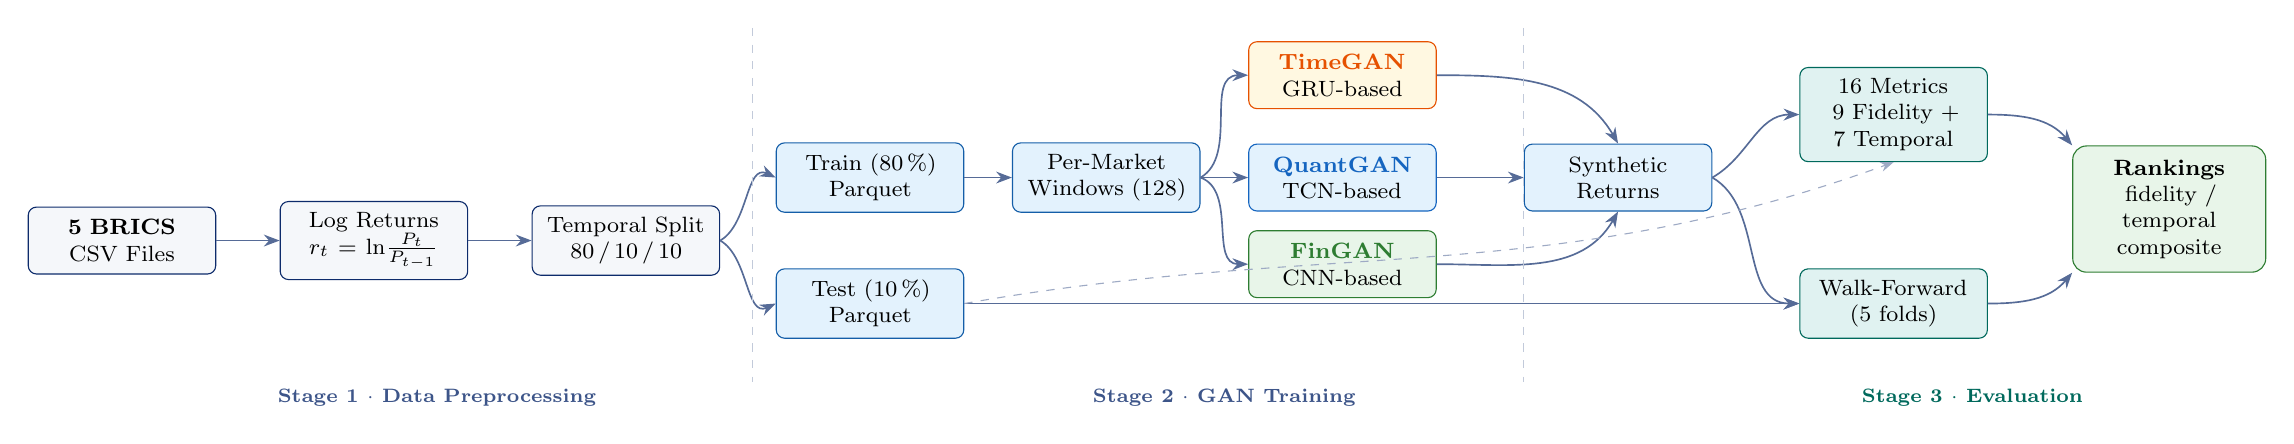
\begin{tikzpicture}[
  every node/.style={font=\footnotesize},
  pp/.style={rectangle, rounded corners=3pt, draw=Navy, fill=LBg,
             text width=2.1cm, align=center, minimum height=0.85cm, inner sep=4pt},
  sp/.style={rectangle, rounded corners=3pt, draw=Sky!80!black, fill=BBg,
             text width=2.1cm, align=center, minimum height=0.85cm, inner sep=4pt},
  ev/.style={rectangle, rounded corners=3pt, draw=Teal, fill=TealBg,
             text width=2.1cm, align=center, minimum height=0.85cm, inner sep=4pt},
  rk/.style={rectangle, rounded corners=5pt, draw=FGreen, fill=GBg,
             text width=2.1cm, align=center, minimum height=1.1cm, inner sep=5pt},
  arr/.style={-Stealth, semithick, draw=Navy!70},
  sarr/.style={-Stealth, thin, draw=Navy!40, dashed},
]
\node[pp] (csv)  at (0.0,  0.0) {\textbf{5 BRICS}\\CSV Files};
\node[pp] (lr)   at (3.2,  0.0) {Log Returns\\$r_t=\ln\!\tfrac{P_t}{P_{t-1}}$};
\node[pp] (spl)  at (6.4,  0.0) {Temporal Split\\80\,/\,10\,/\,10};
\node[sp] (trn)  at (9.5,  0.8) {Train (80\,\%)\\Parquet};
\node[sp] (tst)  at (9.5, -0.8) {Test (10\,\%)\\Parquet};
\node[sp] (poo)  at (12.5,  0.8) {Per-Market\\Windows (128)};
\node[rectangle,rounded corners=3pt,draw=TGcol,fill=ABg,
      text width=2.1cm,align=center,minimum height=0.85cm,inner sep=4pt]
     (tga) at (15.5,  2.1) {\textcolor{TGcol}{\bfseries TimeGAN}\\GRU-based};
\node[rectangle,rounded corners=3pt,draw=QGcol,fill=BBg,
      text width=2.1cm,align=center,minimum height=0.85cm,inner sep=4pt]
     (qga) at (15.5,  0.8) {\textcolor{QGcol}{\bfseries QuantGAN}\\TCN-based};
\node[rectangle,rounded corners=3pt,draw=FGcol,fill=GBg,
      text width=2.1cm,align=center,minimum height=0.85cm,inner sep=4pt]
     (fga) at (15.5, -0.3) {\textcolor{FGcol}{\bfseries FinGAN}\\CNN-based};
\node[sp] (syn)  at (19.0,  0.8) {Synthetic\\Returns};
\node[ev] (sfm)  at (22.5,  1.6) {16 Metrics\\9 Fidelity + 7 Temporal};
\node[ev] (wfv)  at (22.5, -0.8) {Walk-Forward\\(5 folds)};
\node[rk] (rnk)  at (26.0,  0.4) {\textbf{Rankings}\\fidelity / temporal\\composite};
\draw[arr] (csv.east) -- (lr.west);
\draw[arr] (lr.east)  -- (spl.west);
\draw[arr] (spl.east) to[out= 30,in=155] (trn.west);
\draw[arr] (spl.east) to[out=-30,in=205] (tst.west);
\draw[arr] (trn.east) -- (poo.west);
\draw[arr] (poo.east) to[out= 30,in=180] (tga.west);
\draw[arr] (poo.east) --                 (qga.west);
\draw[arr] (poo.east) to[out=-20,in=180] (fga.west);
\draw[arr] (tga.east) to[out=  0,in=120] (syn.north);
\draw[arr] (qga.east) --                 (syn.west);
\draw[arr] (fga.east) to[out=  0,in=240] (syn.south);
\draw[arr]  (syn.east) to[out= 30,in=180] (sfm.west);
\draw[arr]  (syn.east) to[out=-30,in=180] (wfv.west);
\draw[arr]  (tst.east) --                 (wfv.west);
\draw[sarr] (tst.east) to[out=10,in=200]  (sfm.south);
\draw[arr] (sfm.east) to[out=0,in=130] (rnk.north west);
\draw[arr] (wfv.east) to[out=0,in=230] (rnk.south west);
\node[font=\scriptsize\bfseries,text=Navy!80]  at ( 4.0,-2.0) {Stage 1 $\cdot$ Data Preprocessing};
\node[font=\scriptsize\bfseries,text=Navy!80]  at (14.0,-2.0) {Stage 2 $\cdot$ GAN Training};
\node[font=\scriptsize\bfseries,text=Teal]     at (23.5,-2.0) {Stage 3 $\cdot$ Evaluation};
\draw[very thin,dashed,Navy!25] ( 8.0, 2.7) -- ( 8.0,-1.8);
\draw[very thin,dashed,Navy!25] (17.8, 2.7) -- (17.8,-1.8);
\end{tikzpicture}
}
\end{center}

\vspace{6pt}
\begin{multicols}{2}
\small

\navybox{Stage 1 --- Data Preprocessing}{%
Raw price CSVs are converted to daily log returns $r_t = \ln(P_t/P_{t-1})$. Dates are parsed and sorted chronologically. A strict temporal 80/10/10 split ensures no future data leaks into training. Files saved as Parquet for efficient I/O.}

\skybox{Stage 2 --- GAN Training}{%
Each 80\% training file is sliced into 128-step sliding windows. Three GAN families are each trained \emph{independently per market} (15 models: 3 GANs $\times$ 5 markets). No cross-market data mixing. The shuffled control is injected alongside model outputs at evaluation time.}

\columnbreak

\tealbox{Stage 3 --- Evaluation}{%
Generated synthetic series are compared with real test-set returns on 16 stylized-fact metrics (9 Fidelity + 7 Temporal). Walk-forward re-trains each model on 5 rolling folds. Final output: fidelity\_rank, temporal\_rank, composite\_rank, and fold-level mean\,$\pm$\,std. Pooled downstream utility (QLIKE, Kupiec, Christoffersen) is computed once on the combined 5-market test set.}

\end{multicols}

\clearpage

%% ─── ED Table 3: Architecture Comparison ────────────────────────────────────
\pagehead{Extended Data Table 3 --- Architecture Comparison}
         {TimeGAN $\cdot$ QuantGAN $\cdot$ FinGAN side by side}

\vspace{4pt}
{\small
\begin{tabularx}{\linewidth}{@{}lXXX@{}}
\toprule
 & \textbf{\textcolor{TGcol}{TimeGAN}} & \textbf{\textcolor{QGcol}{QuantGAN}} & \textbf{\textcolor{FGcol}{FinGAN}} \\
\midrule
Core architecture & 4-phase (encoder + supervisor + GAN) using GRU & TCN-based WGAN-GP & CNN deconvolution WGAN-GP \\
Temporal mechanism & Recurrent (GRU): processes each step in order, gating what to remember & Dilated convolutions: parallel look at all time scales simultaneously & Transposed convolutions: upsamples from short noise vector to full sequence \\
Training loss & BCE + moment-matching; 4 separate training phases & WGAN-GP (single phase); $n_\text{critic}=5$, $\lambda_\text{gp}=10$ & WGAN-GP (single phase); $n_\text{critic}=5$, $\lambda_\text{gp}=10$ \\
Literature reference & Yoon et al.\ (2019, NeurIPS)\tcite{4} & Wiese et al.\ (2020, \textit{Quant.\ Finance})\tcite{5} & This paper (custom) \\
Key hyperparameters & hidden\_dim=24, num\_layers=3, lr=1e-3 & noise\_dim=100, lr=1e-4, 3 TCN blocks & base\_channels=64, lr=1e-4, 3 ConvTranspose1d \\
seq\_len constraint & Any length & Any length & Must be divisible by 8 \\
Inductive bias & Temporal ordering matters step-by-step; GARCH-like persistence via GRU hidden state & Multi-scale patterns (short + long memory); dilations cover intraday/weekly/monthly simultaneously & Generate from compressed noise like image GANs; hierarchical refinement from coarse to fine \\
Normalisation & MinMax $[0,1]$ & MinMax $[-1,1]$ & MinMax $[-1,1]$ \\
Current training budget & epochs=5 (\textcolor{DRed}{far too low}) & --- & --- \\
\bottomrule
\end{tabularx}}

\vspace{6pt}
\begin{multicols}{2}
\small

\navybox{WGAN-GP shared settings (QuantGAN \& FinGAN)}{%
\textbf{Why $n_\text{critic}=5$:} the critic must accurately estimate the Wasserstein distance before the generator uses the gradient signal. Fewer than 5 updates per generator step leaves the critic under-fitted, providing a biased gradient. Gulrajani et al.\ (2017)\tcite{3} establish this as a minimum; CTBench\tcite{16} and SFAG\tcite{28} fix it identically.

\textbf{Why $\lambda_\text{gp}=10$:} values $<5$ allow Lipschitz violations, invalidating the Kantorovich--Rubinstein duality on which WGAN training is based. The value 10 is the standard from Gulrajani et al.\ (2017)\tcite{3} and has not been improved upon in the literature.

\textbf{Why $\beta_1=0$ in Adam:} in adversarial training, the correct gradient direction for the generator reverses each time the critic is updated. Momentum ($\beta_1>0$) accumulates past-direction information and pushes in the wrong direction. Setting $\beta_1=0$ uses only the current gradient.

\textbf{Why LayerNorm in FinGAN critic (not BatchNorm):} the gradient penalty $\mathcal{L}_\text{GP}$ requires the gradient norm of the critic at a \emph{single} interpolated point. BatchNorm normalises across the batch, introducing a dependency on other samples in the batch that corrupts the gradient norm calculation.}

\columnbreak

\tealbox{TimeGAN four-phase training}{%
\textbf{Phase 1 --- Autoencoder:} train Embedder $e: \mathcal{X} \to \mathcal{H}$ and Recovery $\hat{r}: \mathcal{H} \to \mathcal{X}$. Loss: $\|X - \hat{r}(e(X))\|^2$.

\textbf{Phase 2 --- Supervisor:} train $s: \mathcal{H} \to \hat{\mathcal{H}}$ to predict next latent step. Loss: $\|H_{t+1} - s(H_t)\|^2$. Injects temporal causality into the latent space.

\textbf{Phase 3 --- Joint adversarial:} $z \to G(z) \to s(G(z)) \to \hat{r}(\cdot) \to \tilde{X}$.
\begin{align*}
  \mathcal{L}_G &= \mathcal{L}_U + 100\sqrt{\mathcal{L}_S} + 100\,\mathcal{L}_V \\
  \mathcal{L}_V &= |\mu_H - \mu_{\hat{H}}| + |\sigma_H - \sigma_{\hat{H}}|
\end{align*}

\textbf{Phase 4 --- Fine-tuning:} fine-tune recovery $\hat{r}$ with generated sequences.

\textbf{Current failure:} \texttt{epochs=5} gives each phase $\sim$2 gradient steps. No GRU can form useful representations in 2 steps. All TimeGAN results should be interpreted with this caveat.}

\end{multicols}

\clearpage

%% ─── ED Table 4: Metric Justifications ──────────────────────────────────────
\pagehead{Extended Data Table 4 --- Metric Justifications}
         {Definition $\cdot$ unique contribution $\cdot$ design decision $\cdot$ empirical validation $\cdot$ failure mode}

\begin{multicols}{2}
\small

\tealbox{Fidelity Group: Wasserstein and Energy Distance}{%
\textbf{Wasserstein $W_1$.} $W_1(p,q) = \inf_\gamma \E_{(x,y)\sim\gamma}\|x-y\|$ (Earth Mover's distance). Unique contribution: continuous gradient even when distributions do not overlap; stable under serial dependence. \textit{Rejected alternative:} KS $p$-value --- anti-conservative under serial correlation ($n_\text{eff} \approx n/11$ to $n/31$ for BRICS $|r|$). Empirical validation: shuffled control achieves $W_1 = 0.000\text{e+00}$ (by construction; proves KS and Wasserstein share this blind spot). Failure mode: also permutation-invariant; scores the shuffled control as perfectly matching real data.

\smallskip
\textbf{Energy distance.} $E(P,Q) = 2\E\|X-Y\| - \E\|X-X'\| - \E\|Y-Y'\|$ (Sz\'{e}kely \& Rizzo 2004\tcite{11}). Proper metric on the space of distributions; $E \geq 0$; $E=0 \Leftrightarrow P=Q$. Estimated via subsampled pairs ($n \leq 500$). Empirical validation: shuffled control = 2.97e-05 (near-zero by construction). Failure mode: permutation-invariant.}

\purplebox{Fidelity Group: Quantile MSE and Moment/Tail Diffs}{%
\textbf{Quantile MSE.} $\text{QMSE} = K^{-1}\sum_{k=1}^K [Q_\text{real}(\alpha_k) - Q_\text{syn}(\alpha_k)]^2$, $K=99$. Unique contribution: the only meaningful pointwise comparison between two unaligned distributions (compare by rank, not by index). Captures tail differences at the 1st and 99th percentiles critical for VaR. \textit{Rejected alternative:} pointwise MSE on time-indexed values --- real and synthetic are independently generated; no temporal alignment exists.

\smallskip
\textbf{Moment diffs.} kurtosis\_diff, skewness\_diff, mean\_diff, std\_diff: absolute differences of empirical moments. Included to diagnose which aspect of the marginal a model fails on. All permutation-invariant.

\smallskip
\textbf{Tail index diff.} Hill estimator on the top 5\% of $|r|$: $\hat{\alpha} = k/\sum \log(|r|_{(n-i)}/|r|_{(n-k)})$. Failure mode: Hill estimator has sd 0.52 at $n=995$, falling to 0.035 at $n=4{,}000$ --- the strongest argument for extending the data history.}

\columnbreak

\purplebox{Temporal Group: ACF-MAE Triple}{%
For log-returns $r_t$, compute the sample ACF of $r_t$, $|r_t|$, and $r_t^2$ up to lag 20. Metric: mean absolute error between real and synthetic ACF vectors.

ACF(returns) MAE tests absence of linear predictability (fact 2). ACF($|r|$) and ACF($r^2$) MAE test volatility clustering (Mandelbrot 1963\tcite{9}, fact 3). Shuffled control: 0.043, 0.076, 0.054 --- correctly penalised.

\textit{Why not ARCH-LM?} ACF-MAE is continuous with no saturation regime. ARCH-LM saturates on real data ($|\Delta p| = 0.000000$). ACF-MAE achieves 88\% MC accuracy on simulated GARCH; ARCH-LM achieves 99\% on simulated GARCH but 0\% (ratings the shuffled control as a perfect match) on real data.}

\navybox{Temporal Group: Hurst and Residual Kurtosis}{%
\textbf{Hurst exponent.} $\E[R_n/S_n] \sim c\cdot n^H$, applied to $|r_t|$ (not raw $r_t$; sign flips destroy long memory on raw returns). $H>0.5$: long memory. Metric: $|H_\text{real} - H_\text{syn}|$. Estimated by R/S (Hurst 1951\tcite{23}). Failure mode: sd 0.022 at $n=1{,}000$, 0.004 at $n=4{,}000$.

\textbf{Residual kurtosis.} Fit GARCH(1,1) Gaussian QMLE, extract $\varepsilon_t = r_t/\sigma_t$, report excess kurtosis. Tests fact 7 (Bollerslev 1987\tcite{36}). Gaussian QMLE avoids circularity: a Student-$t$ fit absorbs kurtosis by construction. Real BRICS: MSCI 8.80, NIFTY50 2.12, SHANGHAI 1.79, FTSE 0.93, BOVESPA 0.48.}

\tealbox{Temporal Group: Discriminative AUC}{%
Logistic classifier on 20-day rolling windows. AUC = 0.5 is the optimum (indistinguishability). Ranking metric: $|\text{AUC} - 0.5|$ (not raw AUC). Empirical null: $0.506 \pm 0.084$ (15 seeds, real vs real half-splits). z-score: $(\text{AUC} - 0.506)/0.084$.

\textit{Direction bug found:} ascending rank on raw AUC put 0.30 above 0.50. Fixed by ranking on distance from chance.

\textit{Null shift from CV shuffling:} adding \texttt{shuffle=True} to cross-validation folds moves null from 0.506 to 0.584, because overlapping 20-day windows place near-duplicates in both train and test. Unshuffled CV is correct.}

\end{multicols}

\end{document}
